\documentclass{article}
\usepackage[utf8]{inputenc}
\usepackage{amsfonts}
\usepackage{algorithm2e}
\usepackage{amsmath}
\usepackage[a4paper]{geometry}
\geometry{hscale=0.8,vscale=0.9,centering}
\usepackage{graphicx}
\usepackage{program}
\usepackage{ulem}
\usepackage{xcolor}
\usepackage{pdfpages}
\usepackage{hyperref}

\title{M1 Info – ARC - LAB2}
\author{Olivier HUREAU - Groupe 3}
\date{18/03/2020}

\begin{document}
\maketitle

\section{Dessin de l'automate}

\begin{figure}[!h]
\advance\leftskip+3.5cm
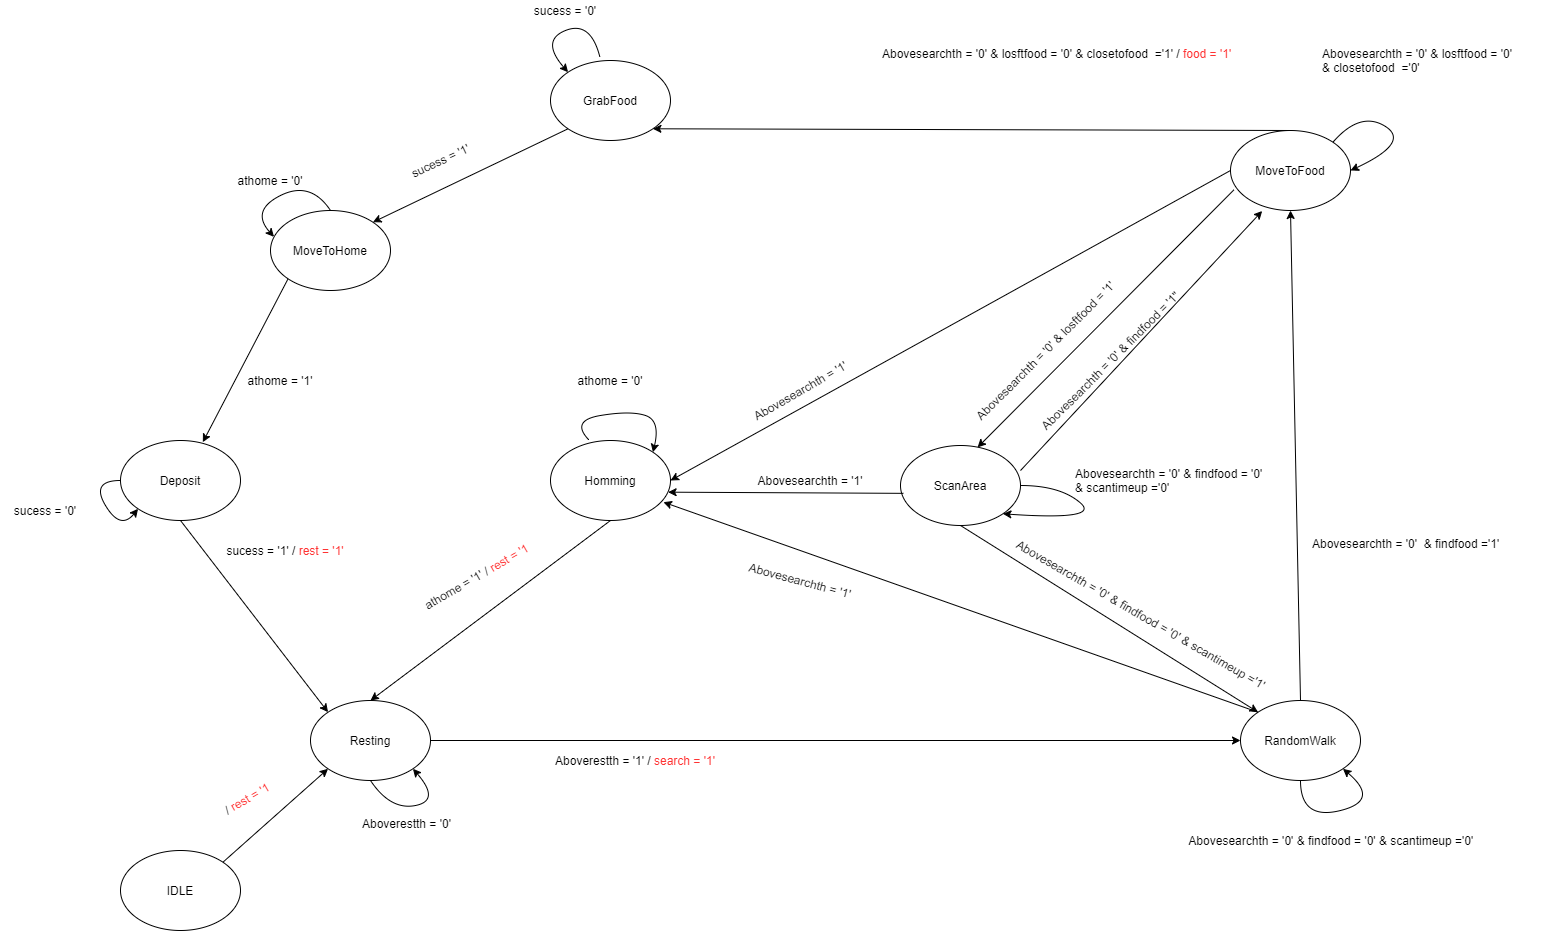
\includegraphics[scale=0.36, angle=-90]{Automate.png}
\caption{Automate du robot}
\end{figure}

\newpage
\section{Description VHDL comportementale}
Le code source est donné en annexe du document (robot.vhd et testRobot.vhd)

\section{TestRobot}
\subsection{Réalisation du test}
Pour tester mon implémentation, j'ai tout d'abord rédigé un tableau des différentes entrées et sorties et des comportements que ceux-ci devais avoir pour toutes les transitions ainsi que les différentes pour y accéder depuis un reset de l'automate.

Dans ce tableau se trouve différentes informations tel que : En rouge :  les inputs que je doit mettre à 1, En bleu : les données que doivent prendre les outputs. 

Ce tableau est fournis en annexe. 
\subsection{Interpretation du test}

Après simulation, on obtiens les différents graphes fournis en annexe. La figure 2 représente la totalité de la simulation. Les figures 3, 4 et 5 sont cette même simulation partitionné. 

Ce que l'on peux observer avec ces différents graphes c'est que notre simulation implémente bien le problème. Les sorties  et la suite d'état correspondent bien à ce qui a était prédit dans notre tableau.

\section{Counter}
Le code source est donné en annexe du document (count.vhd et testCount.vhd)

Après simulation, sur la figure 6 on observe bien que le compteur ne se met en marche uniquement lorsque l'état start est à 1 et le reset fonctionne bien. Le nombre de front montant compté est le bon.

\section{System}
Le programme compile et la simulation se fait, je n'ai pas eu le temps de faire le testbench, je le rendrais plus tard...

En annexe le code.


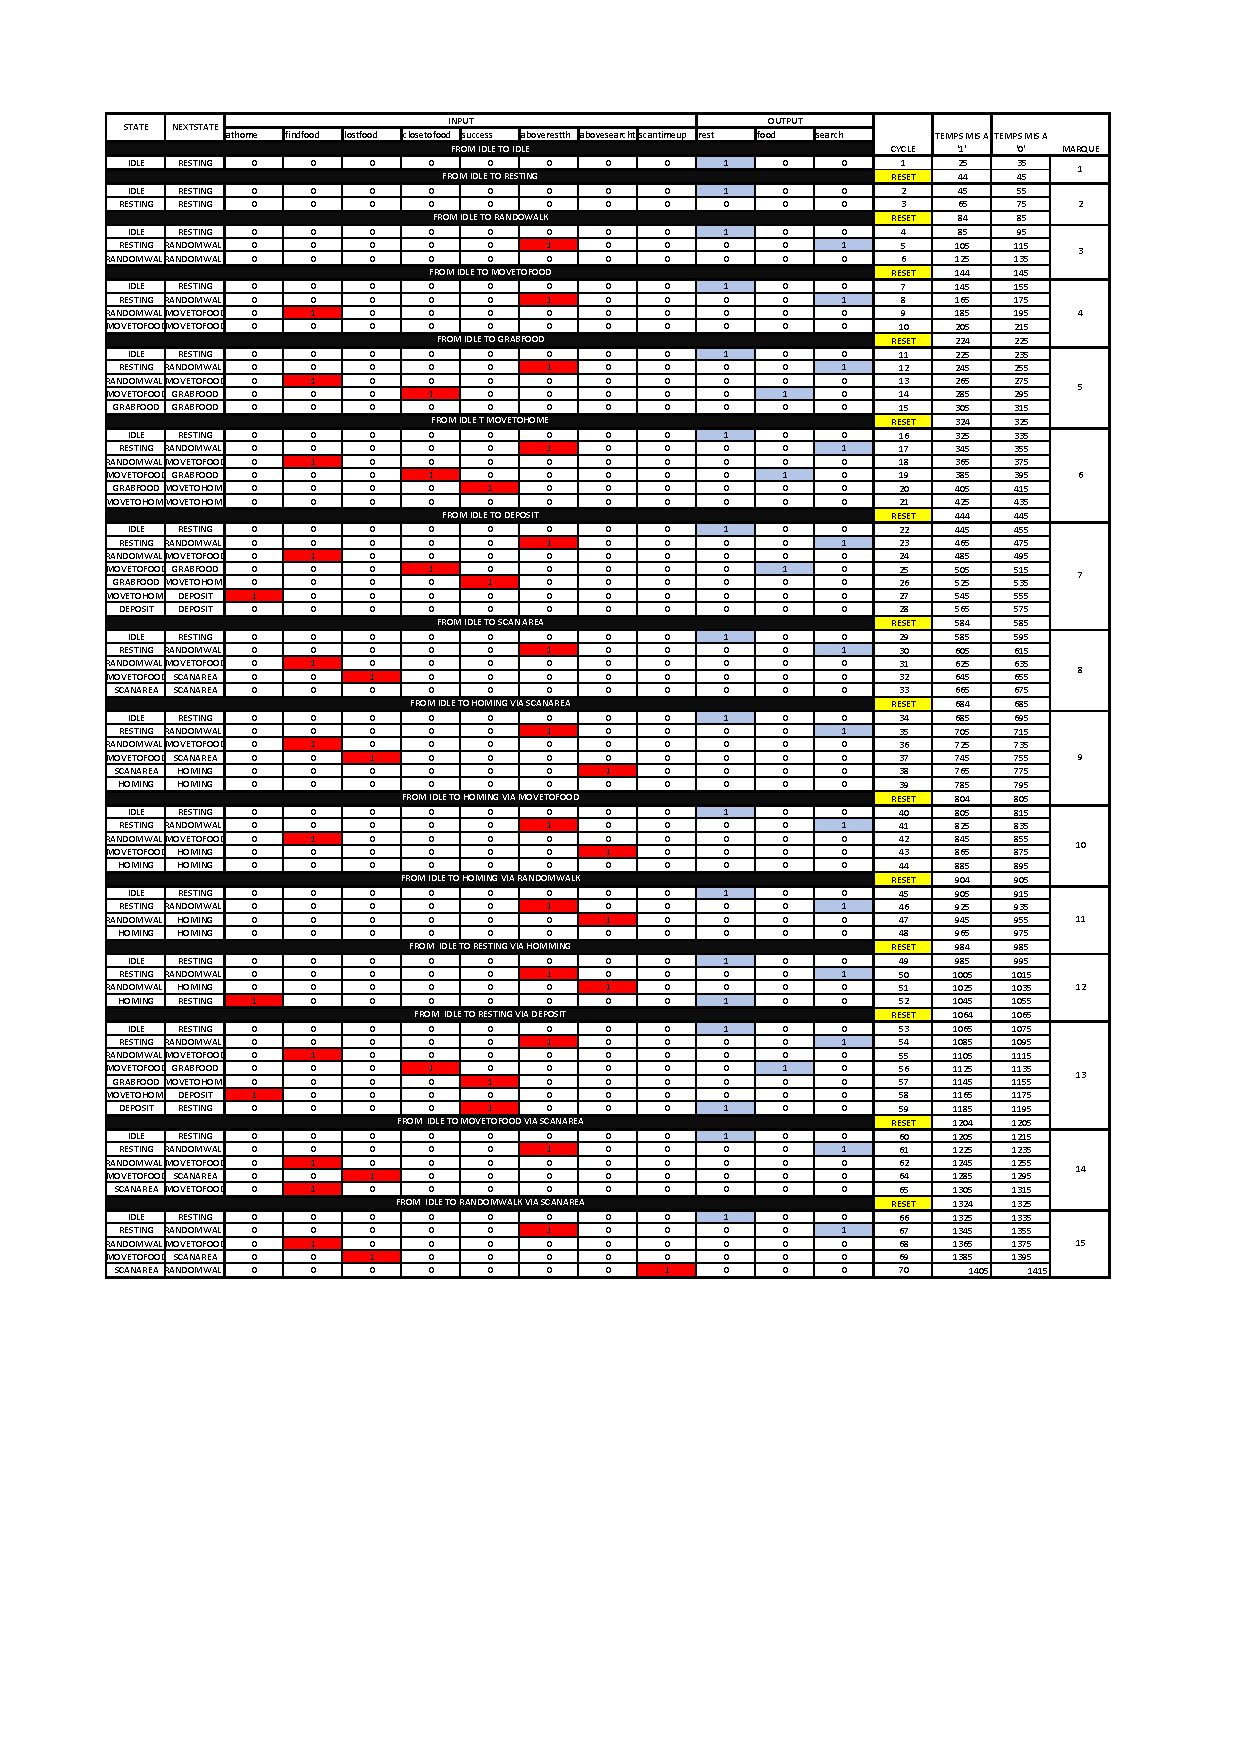
\includepdf{TestBench.pdf}
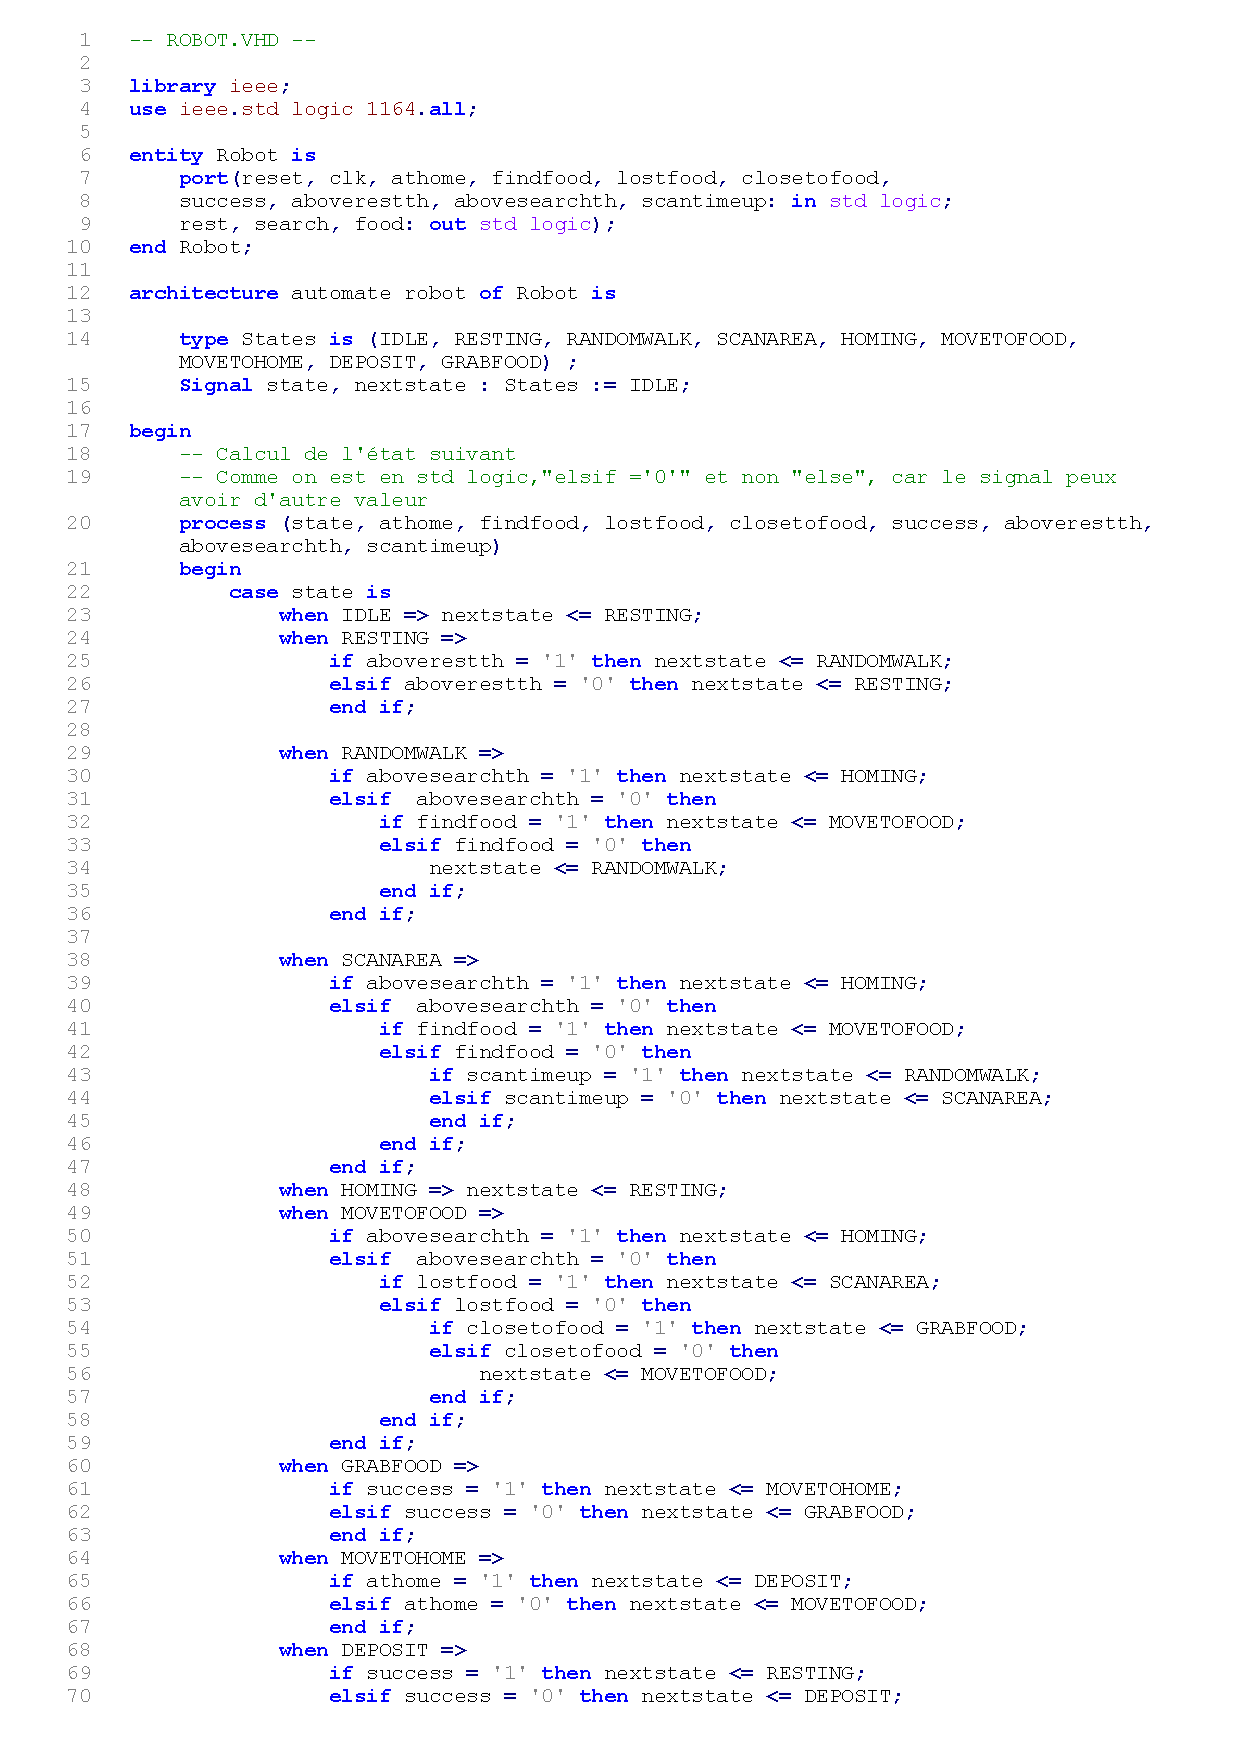
\includepdf{robot.pdf}
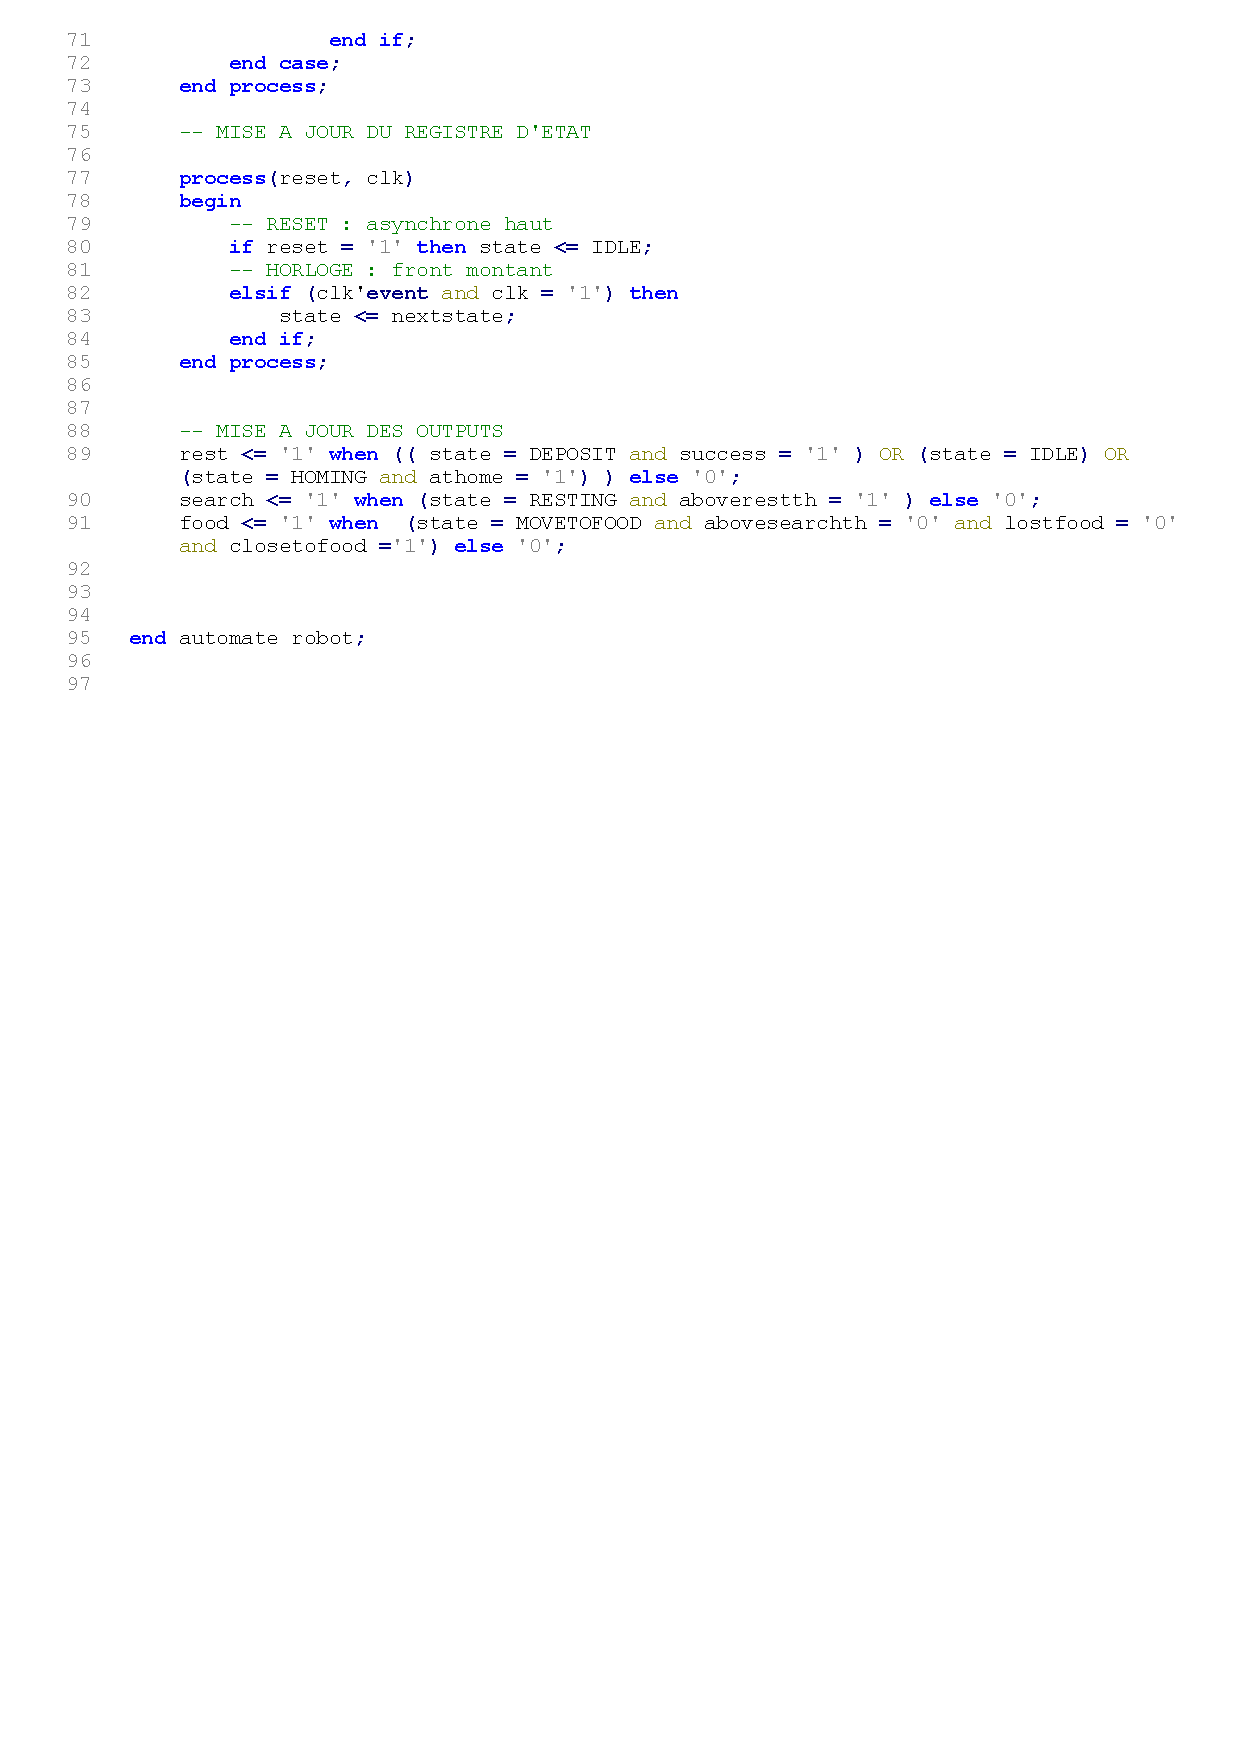
\includepdf{robot2.pdf}
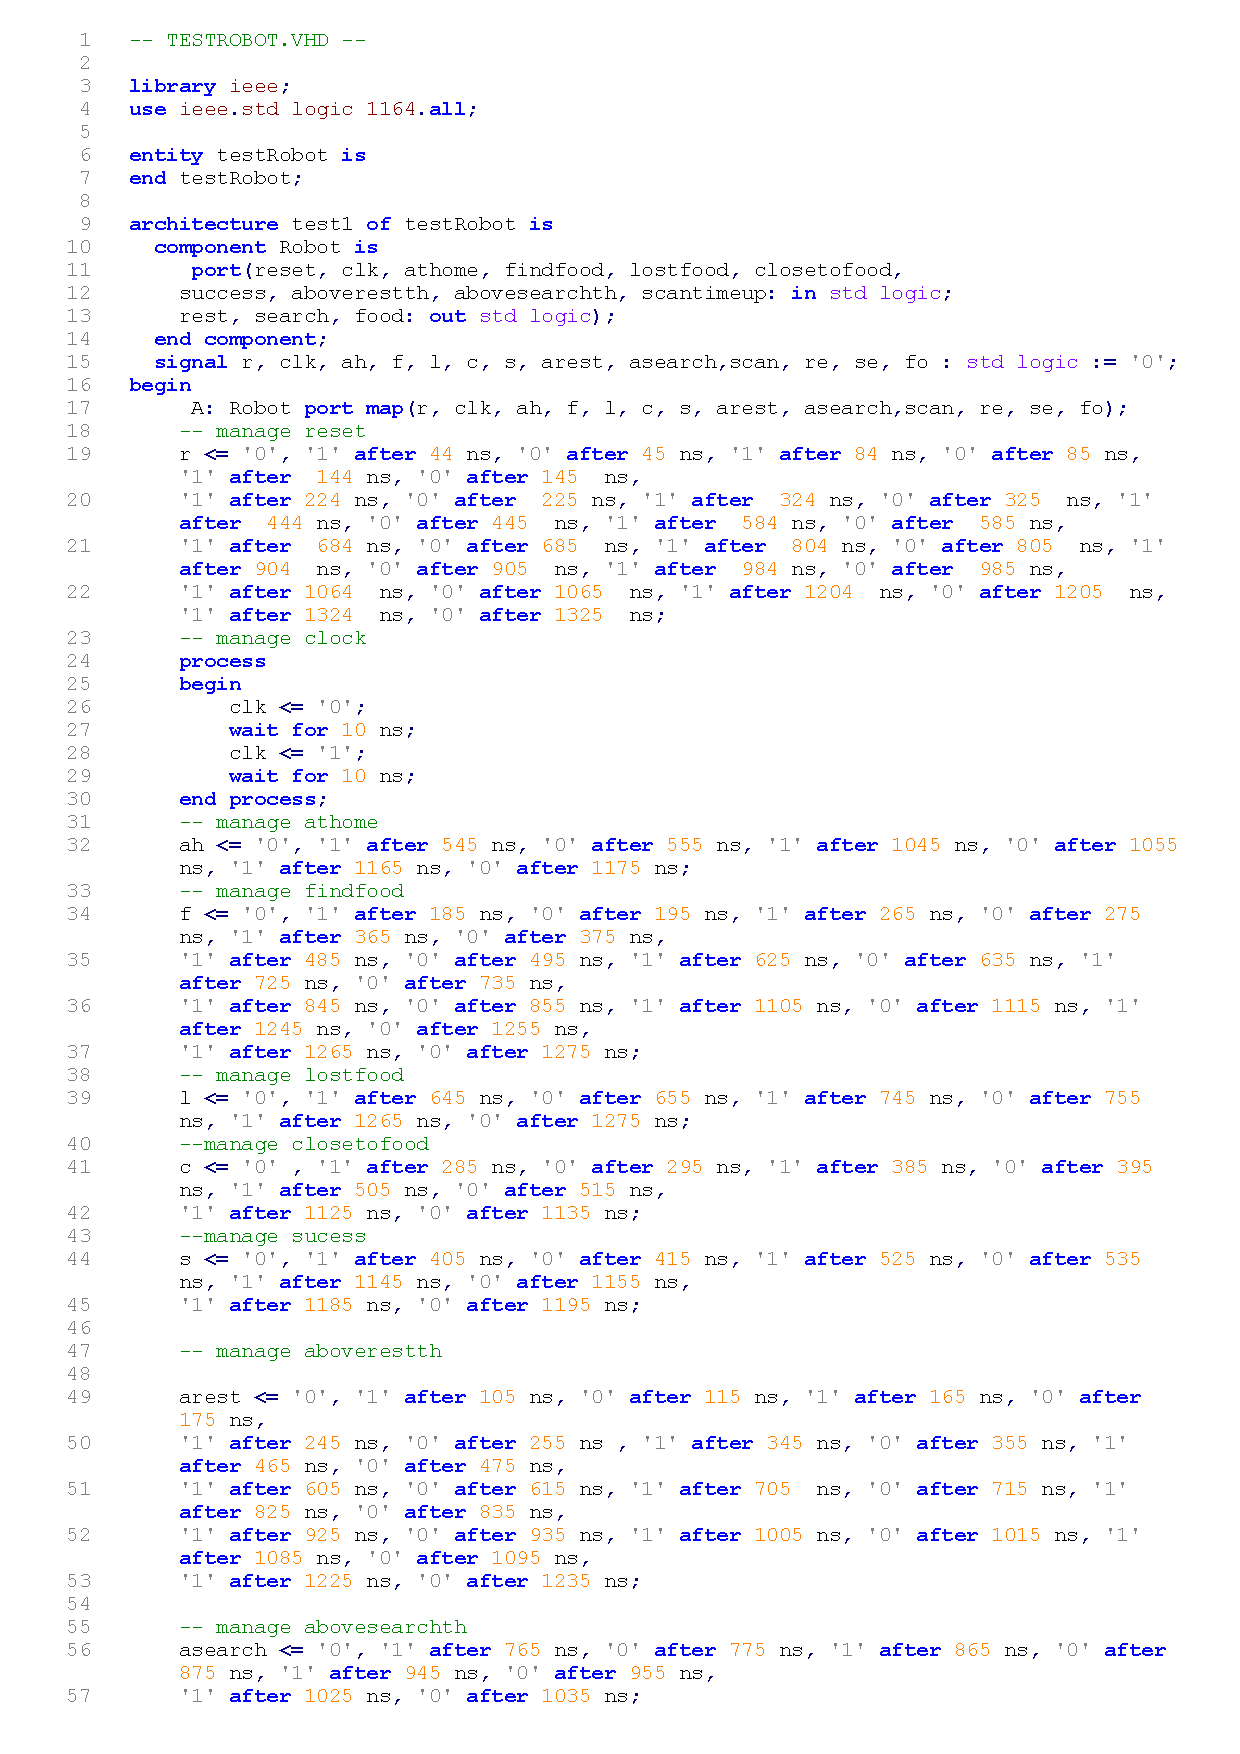
\includepdf{TestRobot.pdf}
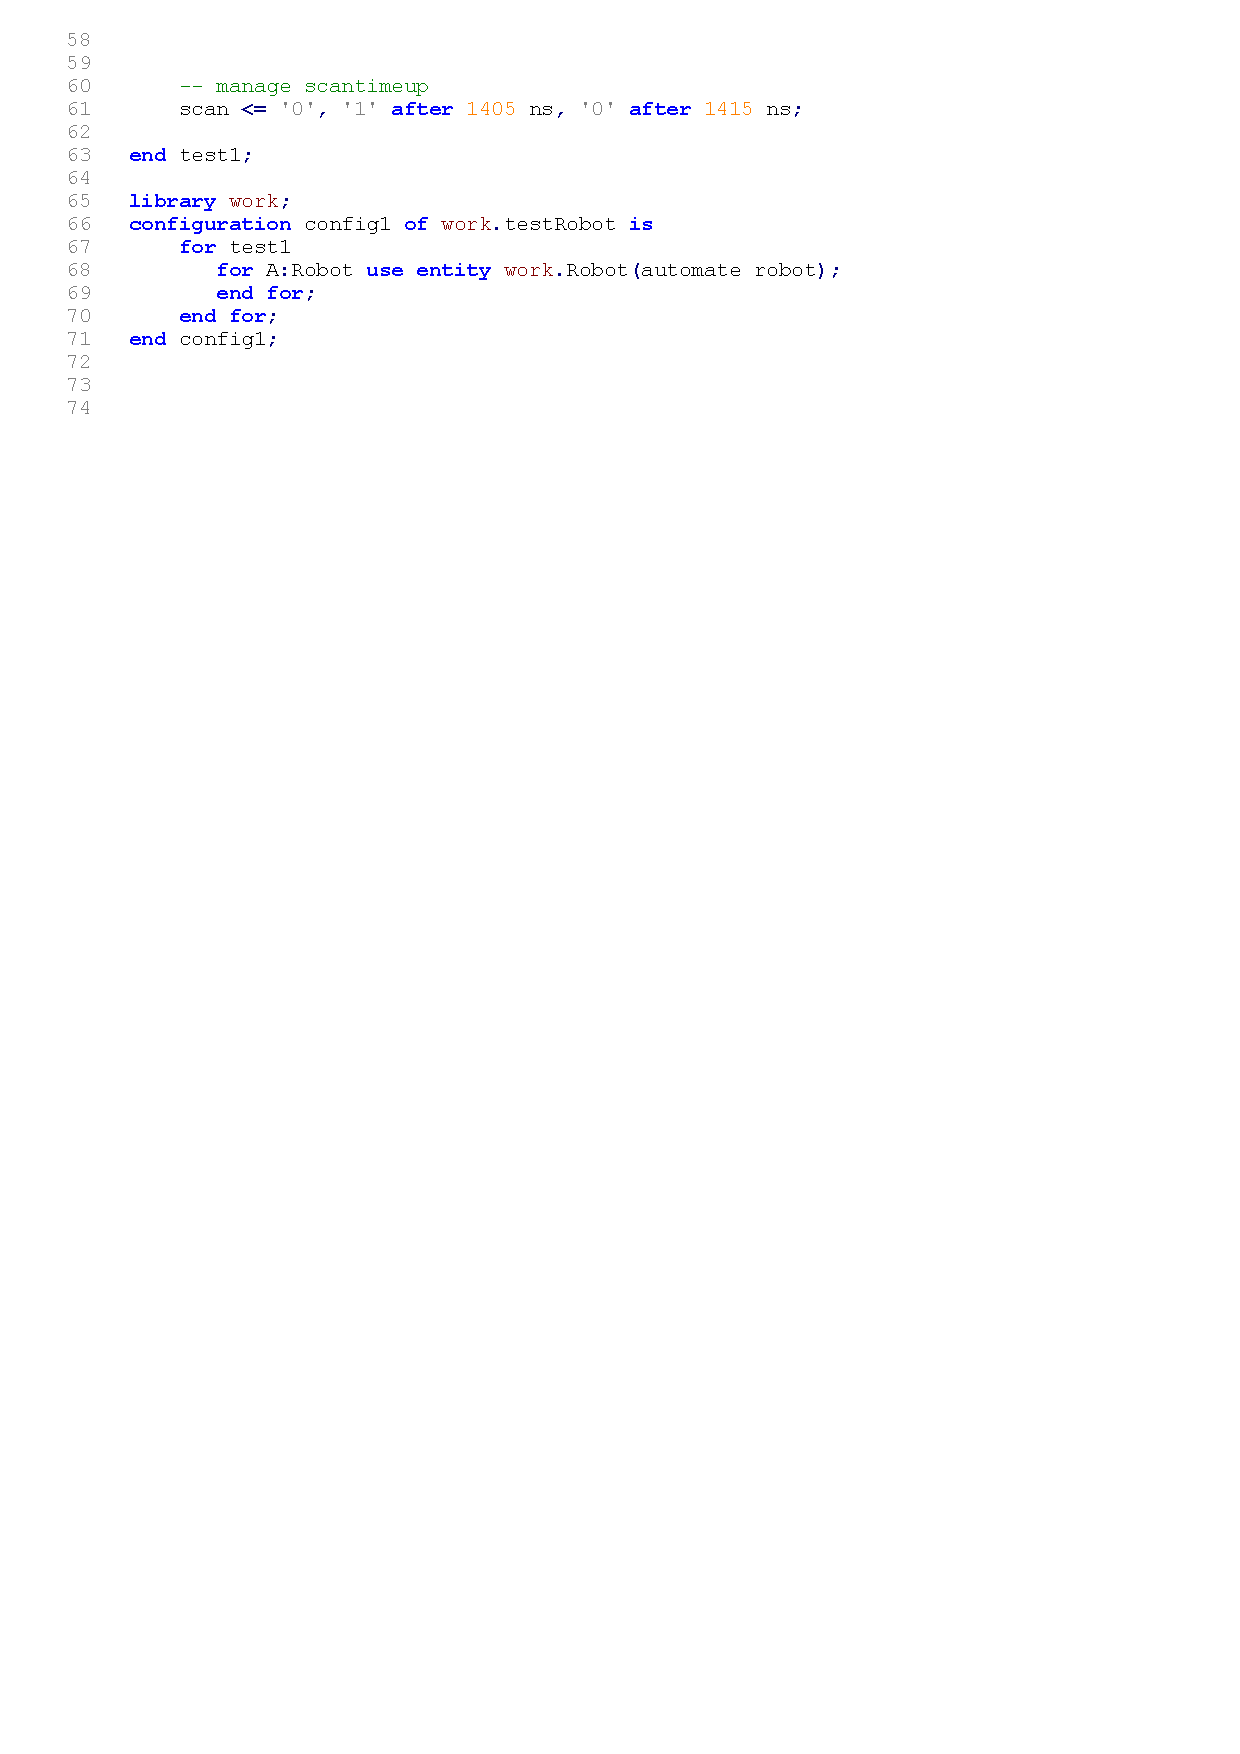
\includepdf{TestRobot2.pdf}

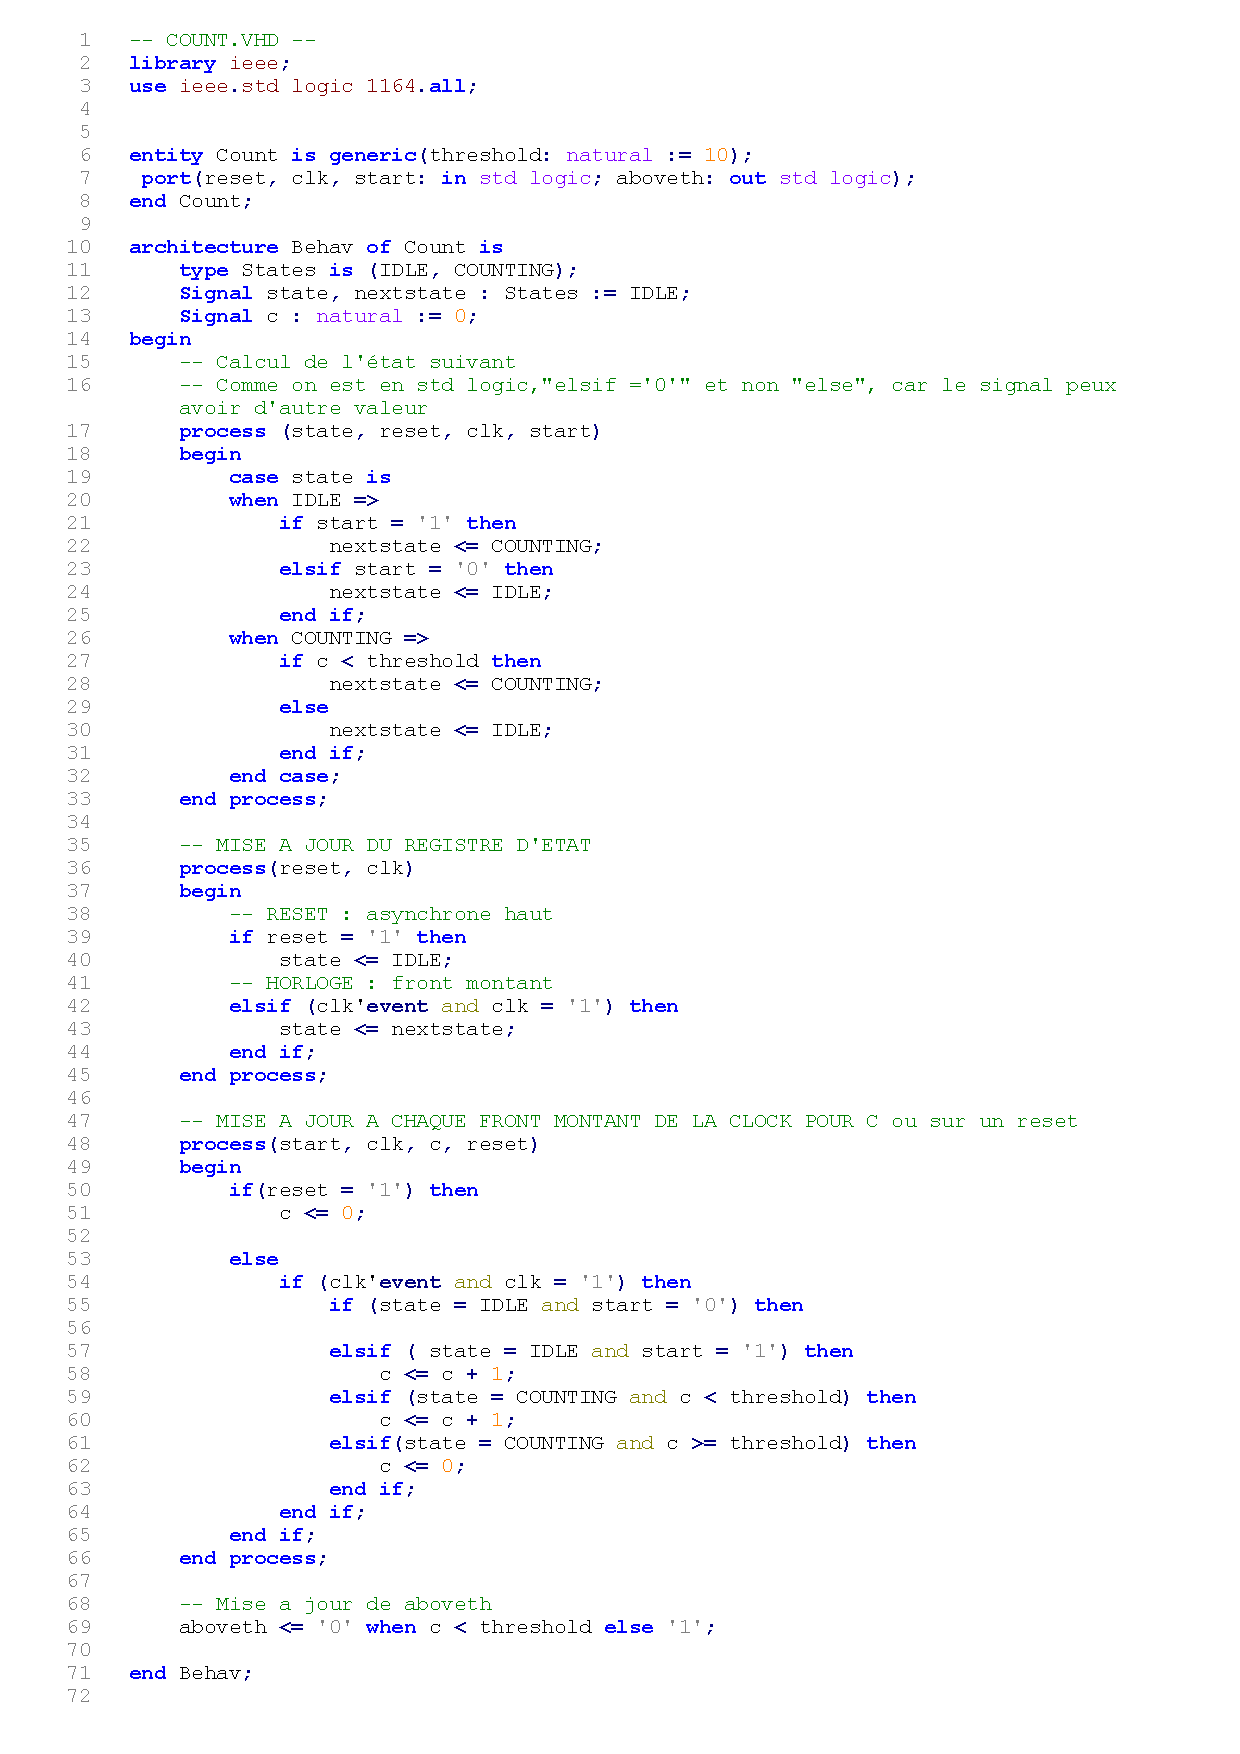
\includepdf{count.pdf}
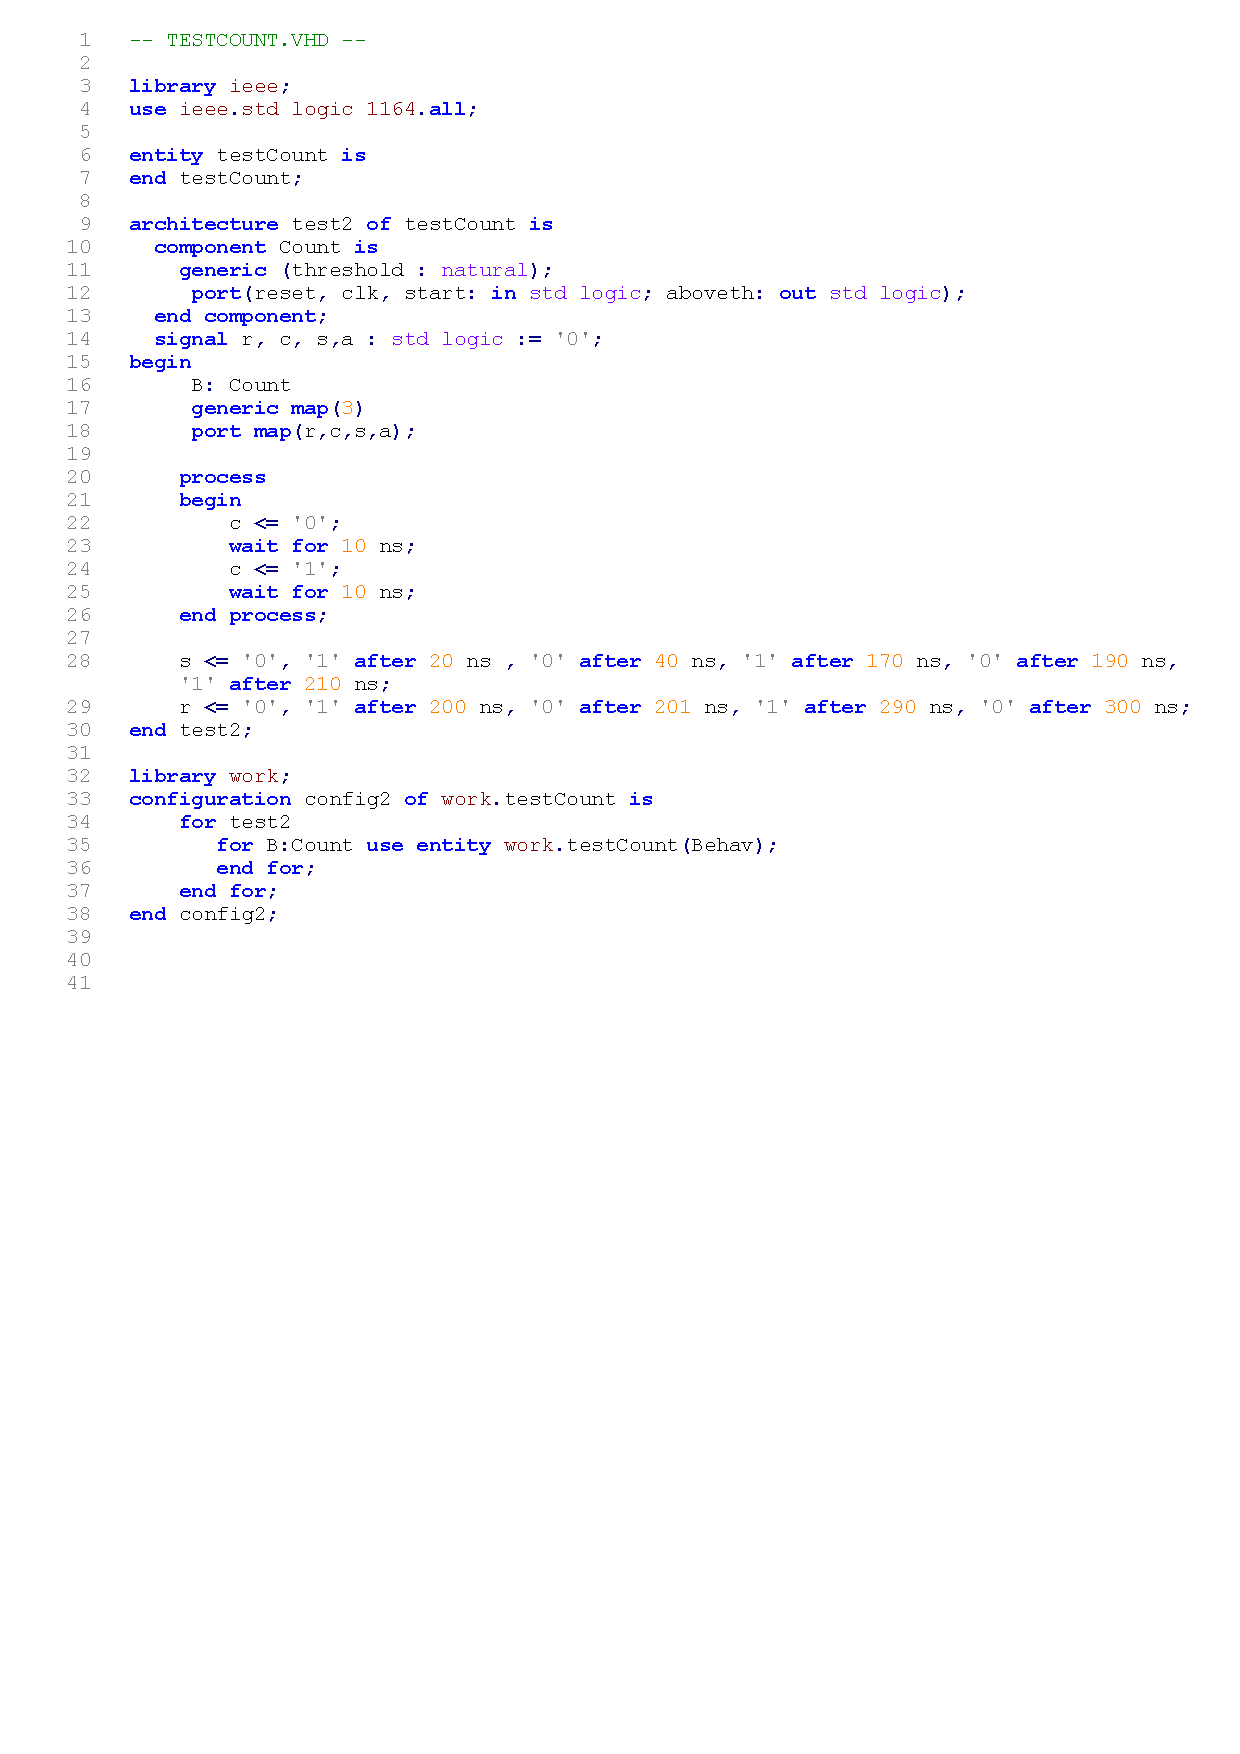
\includepdf{TestCount.pdf}
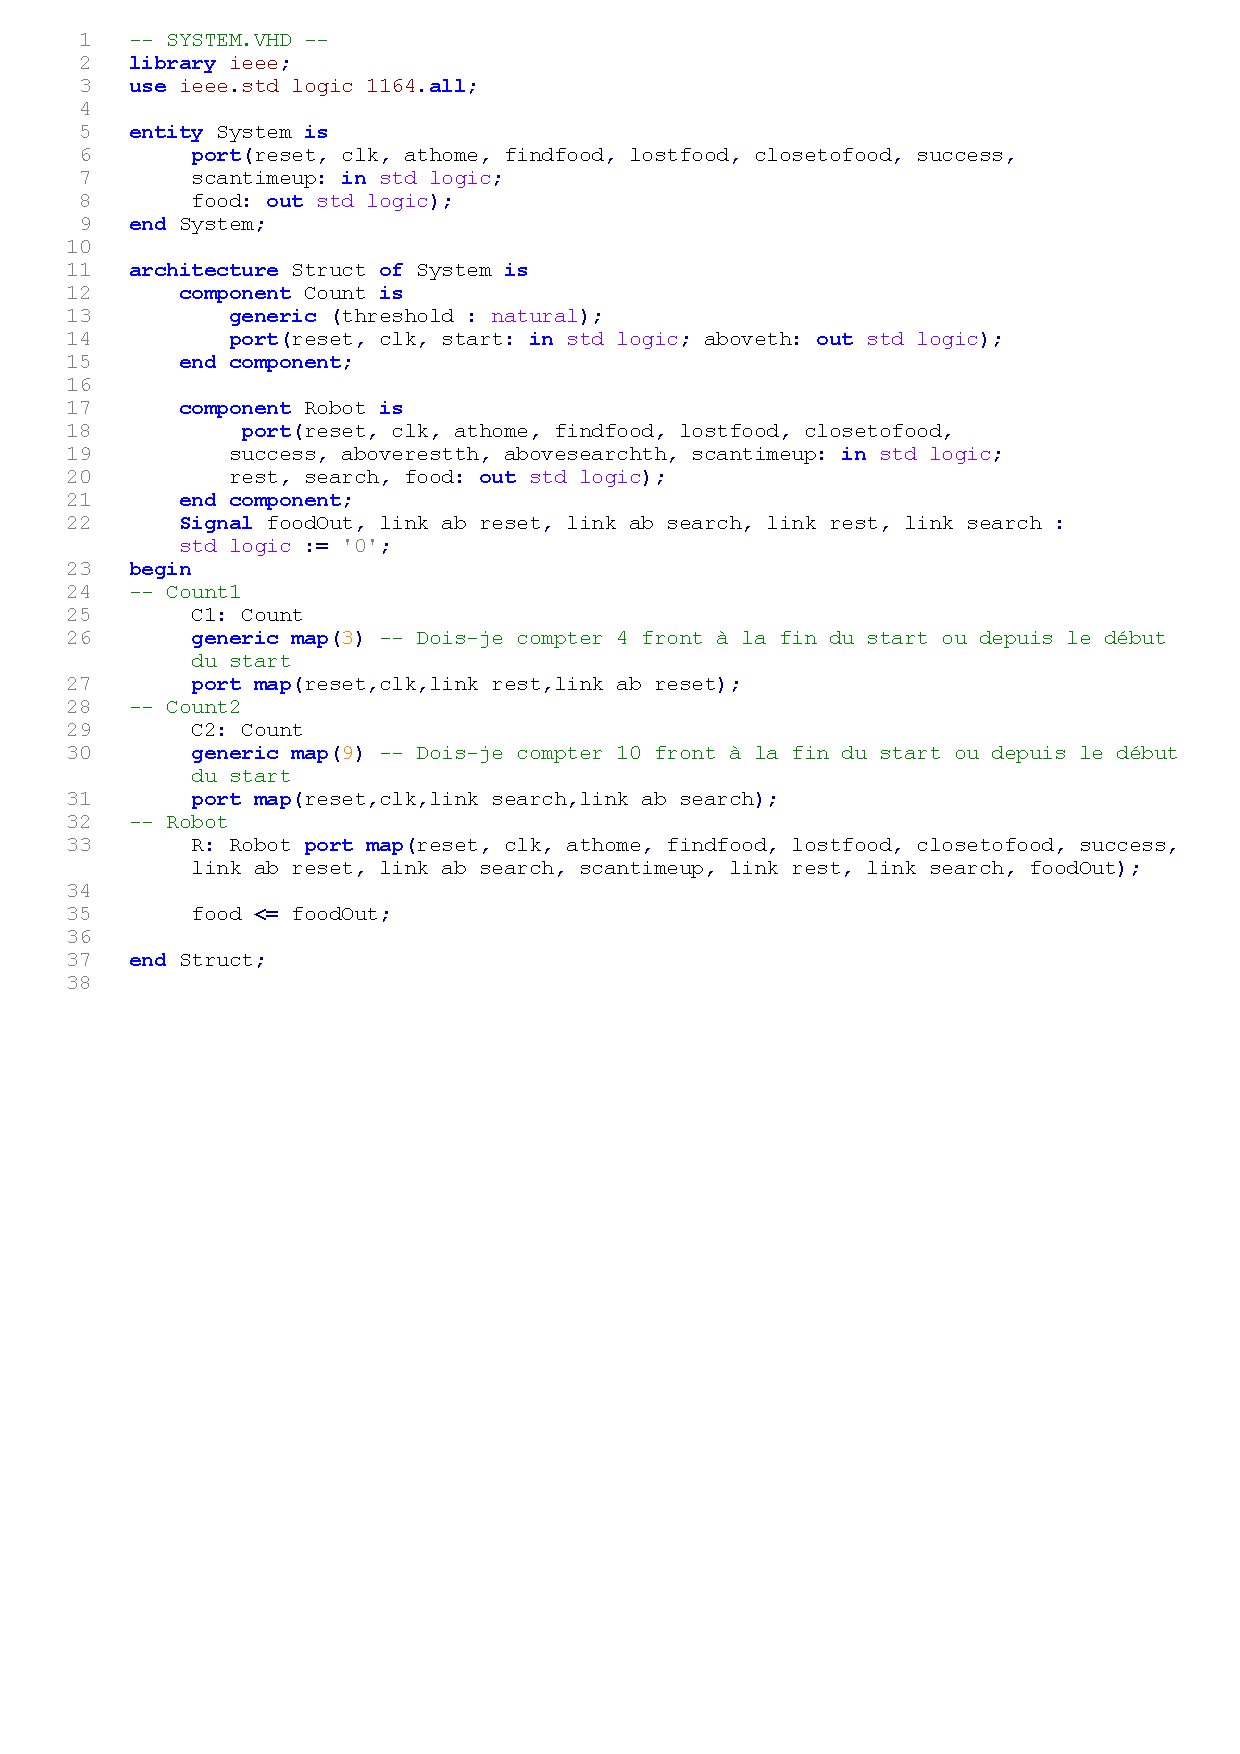
\includepdf{system.pdf}
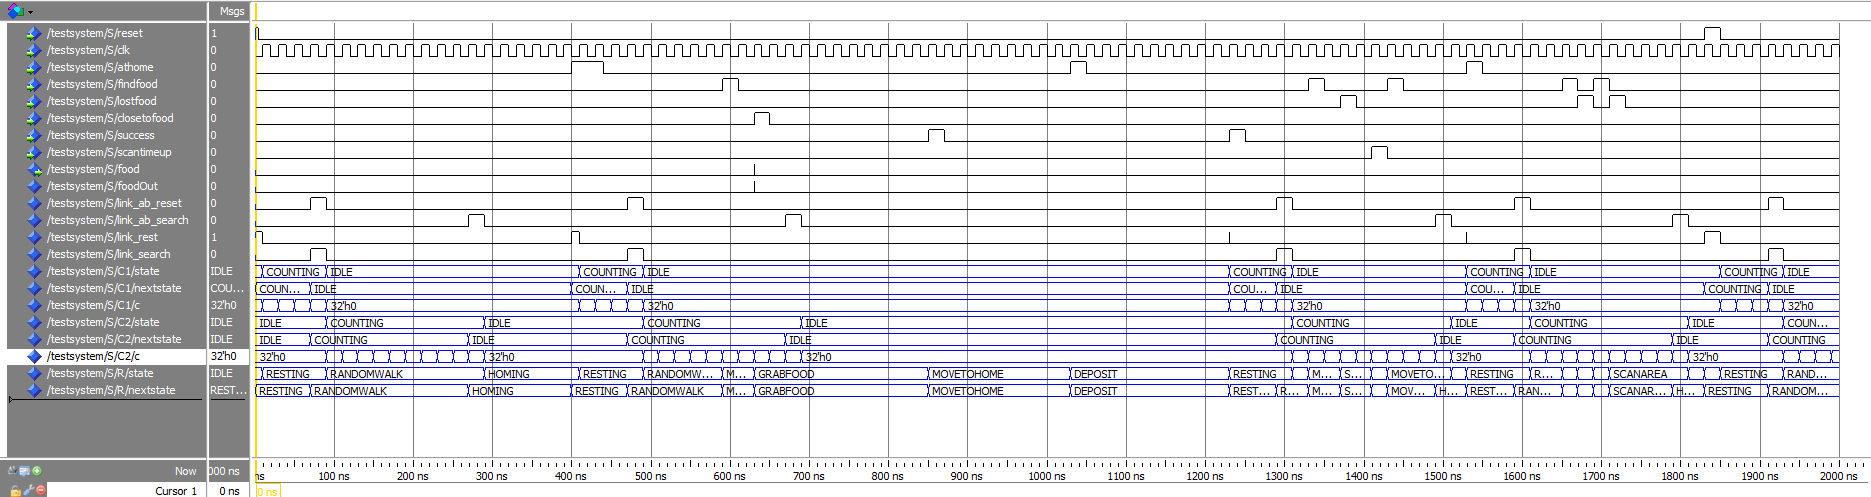
\includepdf{TestSystem.pdf}

\begin{figure}[!h]
\advance\leftskip+6cm
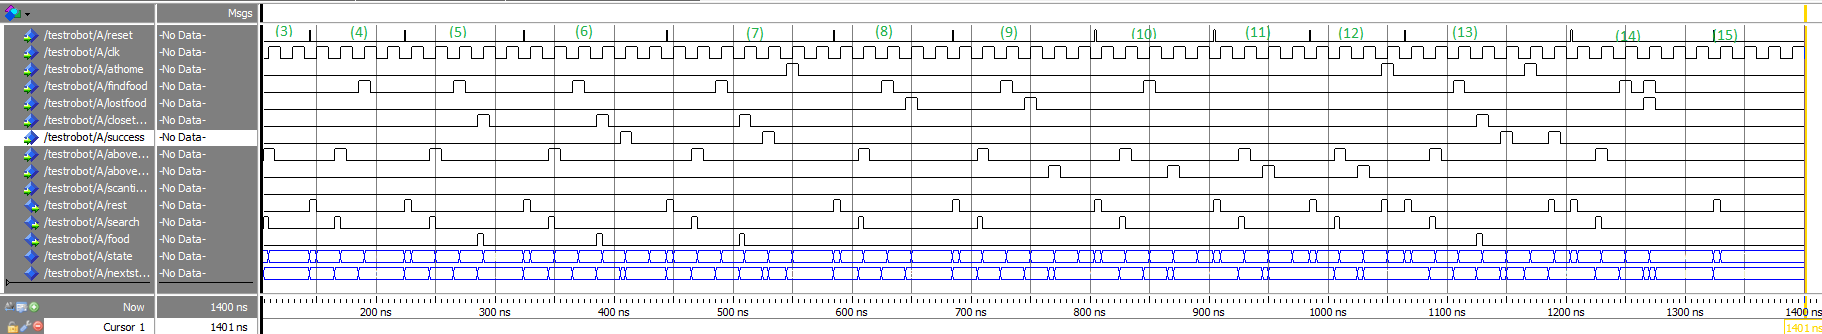
\includegraphics[scale=0.50, angle=-90]{TestRobotMain.PNG}
\caption{Simulation du robot}
\end{figure}

\begin{figure}[!h]
\advance\leftskip+6cm
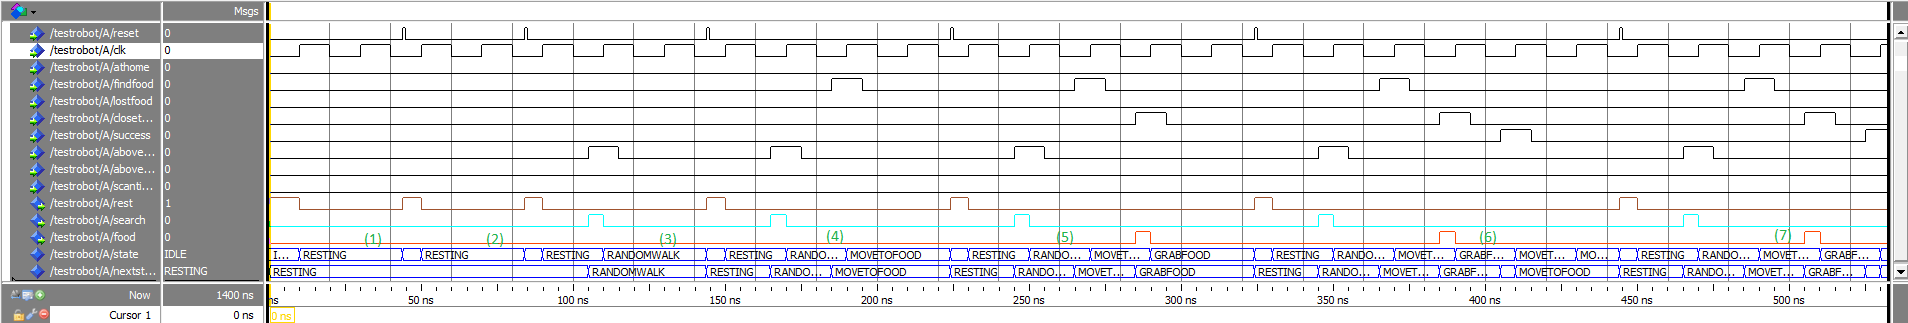
\includegraphics[scale=0.50, angle=-90]{detail_part1.PNG}
\caption{Simulation du robot : 0 ns à 500 ns}
\end{figure}

\begin{figure}[!h]
\advance\leftskip+6cm
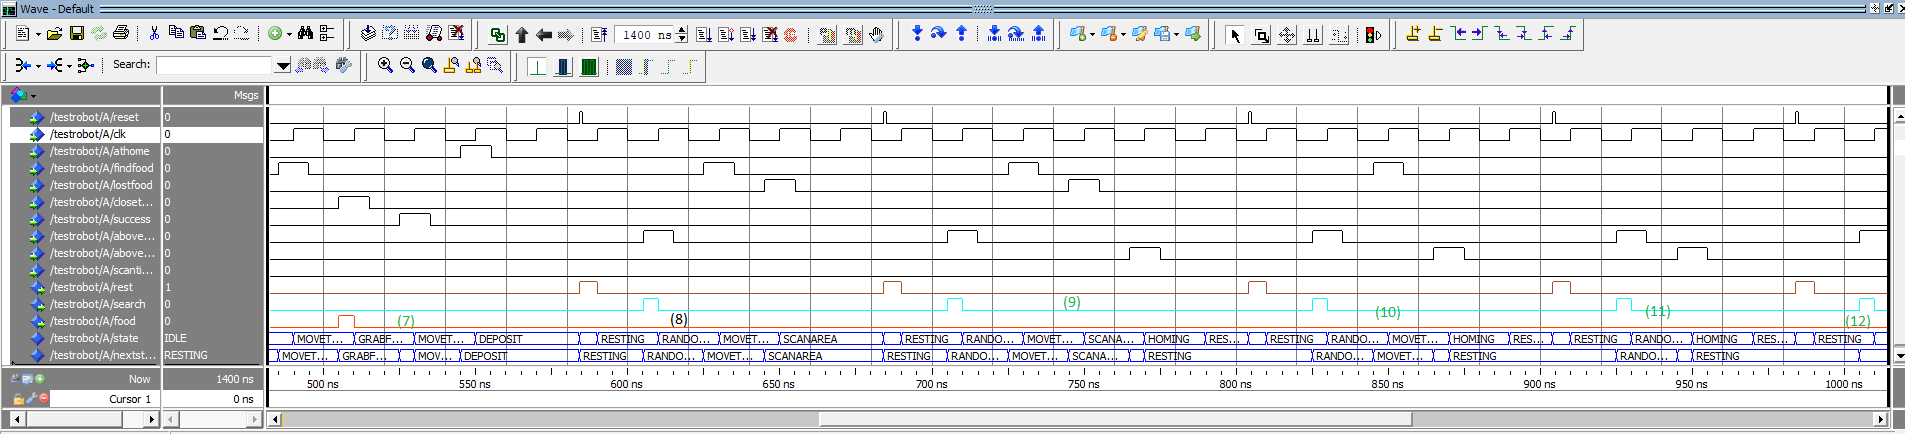
\includegraphics[scale=0.50, angle=-90]{detail_part2.PNG}
\caption{Simulation du robot : 500 ns à 1000 ns}
\end{figure}

\begin{figure}[!h]
\advance\leftskip+6cm
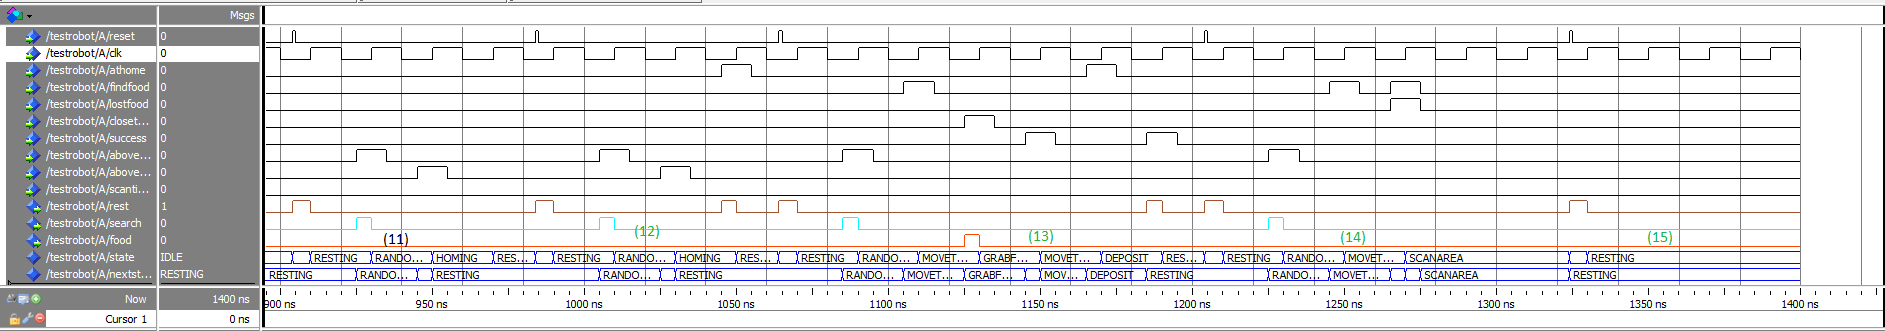
\includegraphics[scale=0.50, angle=-90]{detail_part3.PNG}
\caption{Simulation du robot : 1000 ns à 1500 ns}
\end{figure}

\begin{figure}[!h]
\advance\leftskip+6cm
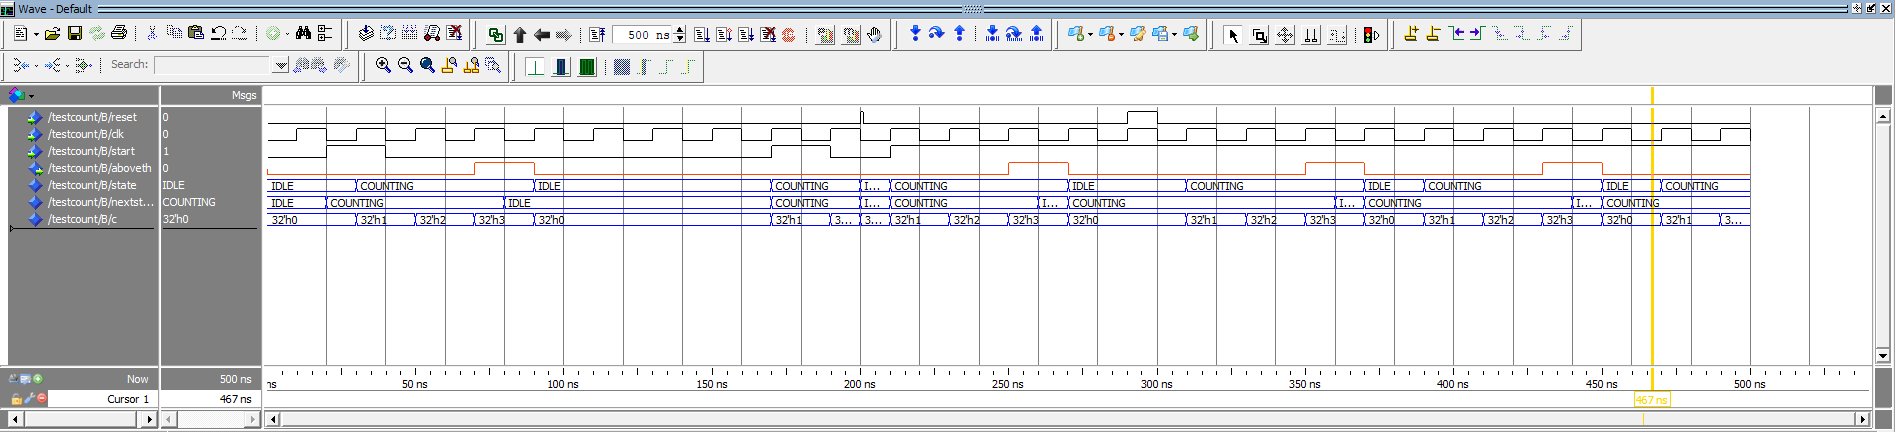
\includegraphics[scale=0.50, angle=-90]{count.PNG}
\caption{Simulation du Count}
\end{figure}

\newpage

\section{Travail effectué après le rendu}
\subsection{Modification du code}
Après le rendu, j'ai continué le travail afin de pouvoir simuler le système complet.

Voici quelques erreurs que j'ai pu trouver :

\begin{itemize}

\item J'ai oublié d'implémenter le fait d'attendre l'entrée 'athome' pour effectuer la transition entre l'état HOMING et l'état RESTING


\item
Ligne 66 du fichier robot.vhd : J'ai écris MOVETOFOOD au lieu de MOVETOHOME


\item
Ligne 17 de count.vhd : mauvaise liste de sensibilité. J'ai donc remplacé 
\begin{verbatim}
process(state, reset, clk, start)
par
process (state, start, c) 
\end{verbatim}

\item
Ligne 37 de count.vhd: J'ai oublié de prendre en compte le signal start pour la mise à jour instantanée des registres. J'ai alors rajouté start a la liste de sensibilité et ajouté le code suivant pour pouvoir détecter un spike :

\begin{verbatim}
if ( (start = '1') and (state = IDLE) )then
	state <= COUNTING;
end if;
\end{verbatim}

Je fournis aussi ci dessous le fichier finale de testSystem.vhd 

Les différentes modifications et le code suplémentaire sont disponnible sur mon github : \url{https://github.com/egobiah/ARC}


\end{itemize}

\subsection{Testbench}
Comme dans le premier testbench, je me suis fixé l'objectif de passer par toutes les transitions et de vérifier que l'enchainement des états est correct. 
\vspace{5mm}
Je réutilise alors le même principe de tableau que précédemment pour calculer mes enchainements cependant désormais d'autres colonnes viennent en complément.

\subparagraph{Déclenchement c1} Cette colonne me permet de calculer  combien de repérer quand-est ce que le signal rest est déclenché et combien de temps dois-je attendre avant de faire une autre action.

\subparagraph{Attente counter} Le nombre de cycle à attendre.

Ci dessous le tableau et la figure 7 représentant le chrono-graphe complet, les figures 8,9,10 et 11 des partitions du chrono-graphe


\includepdf{TestSystem2.pdf}

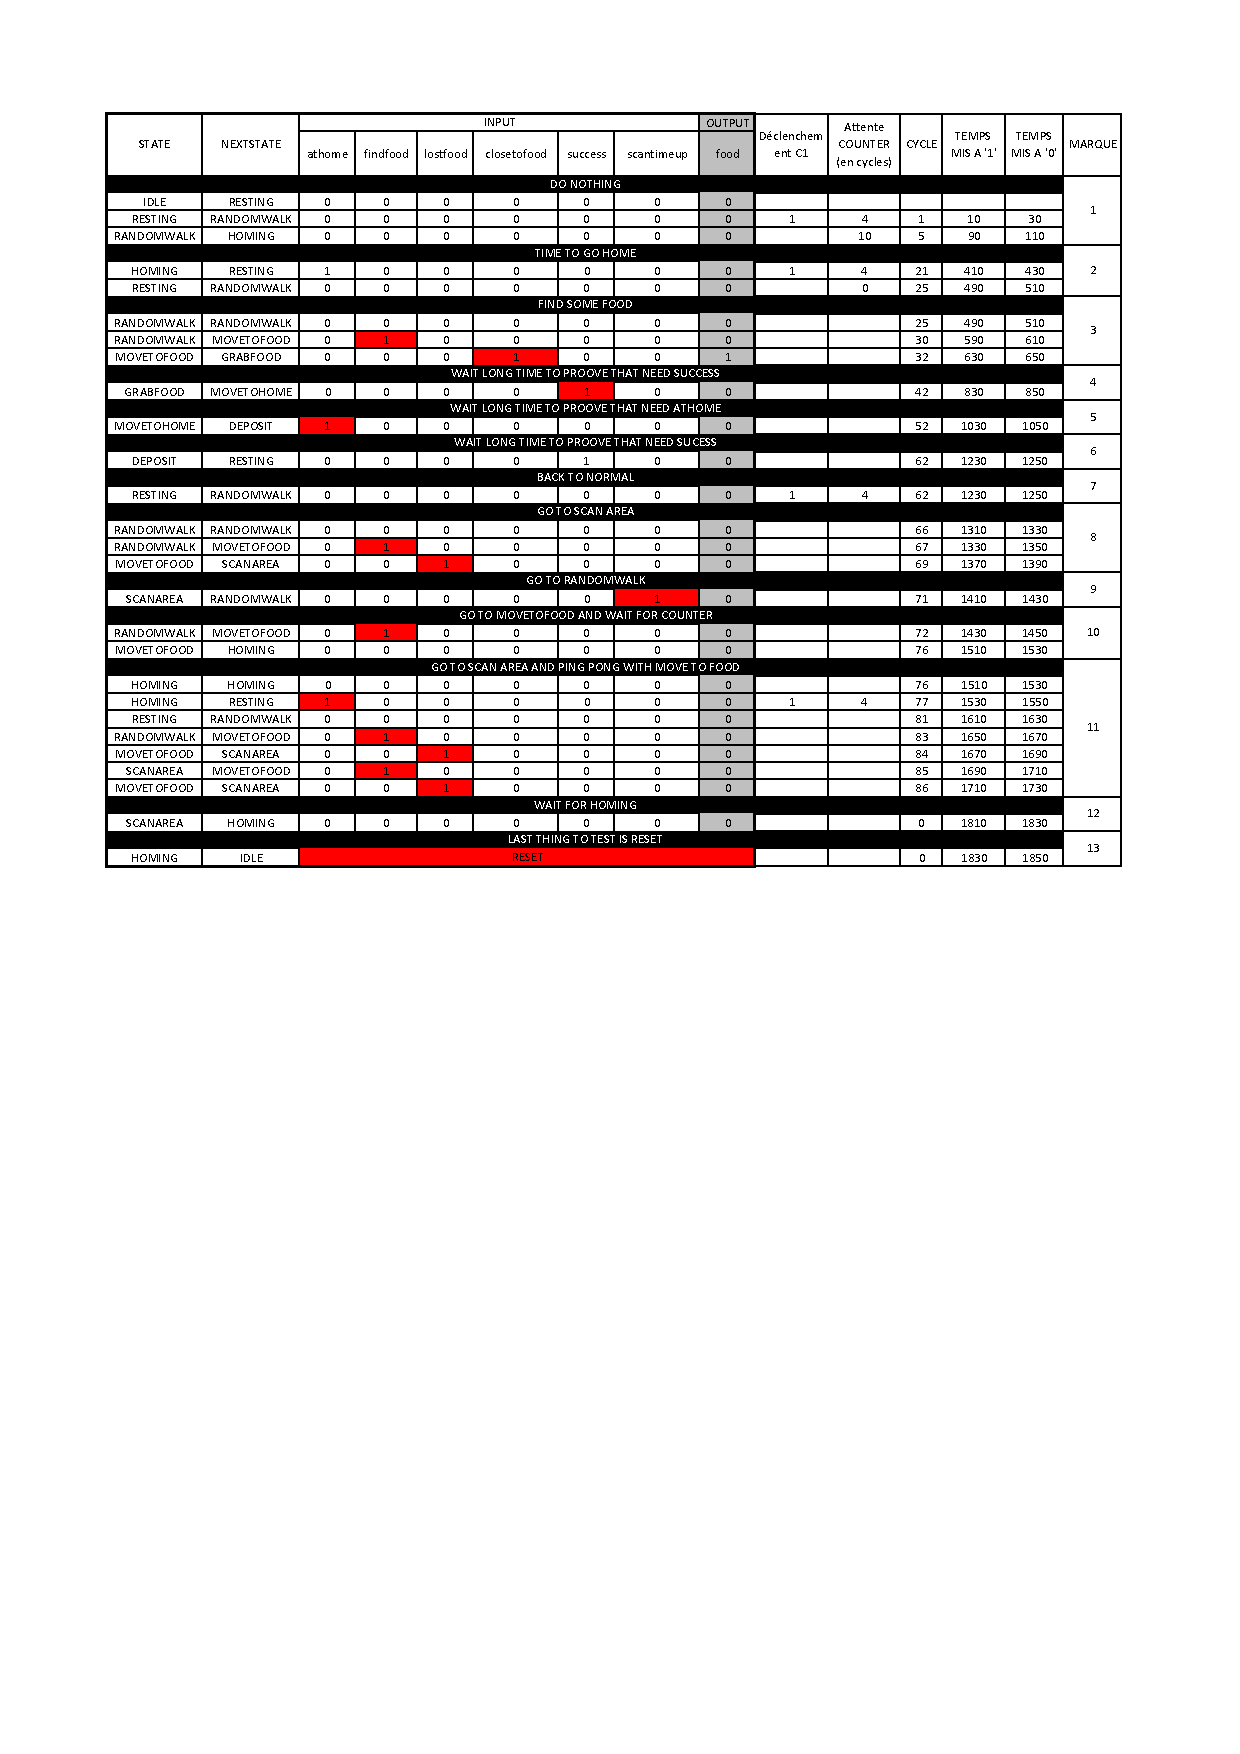
\includepdf{TestBenchSystem.pdf}

\begin{figure}[!h]
\advance\leftskip+6cm
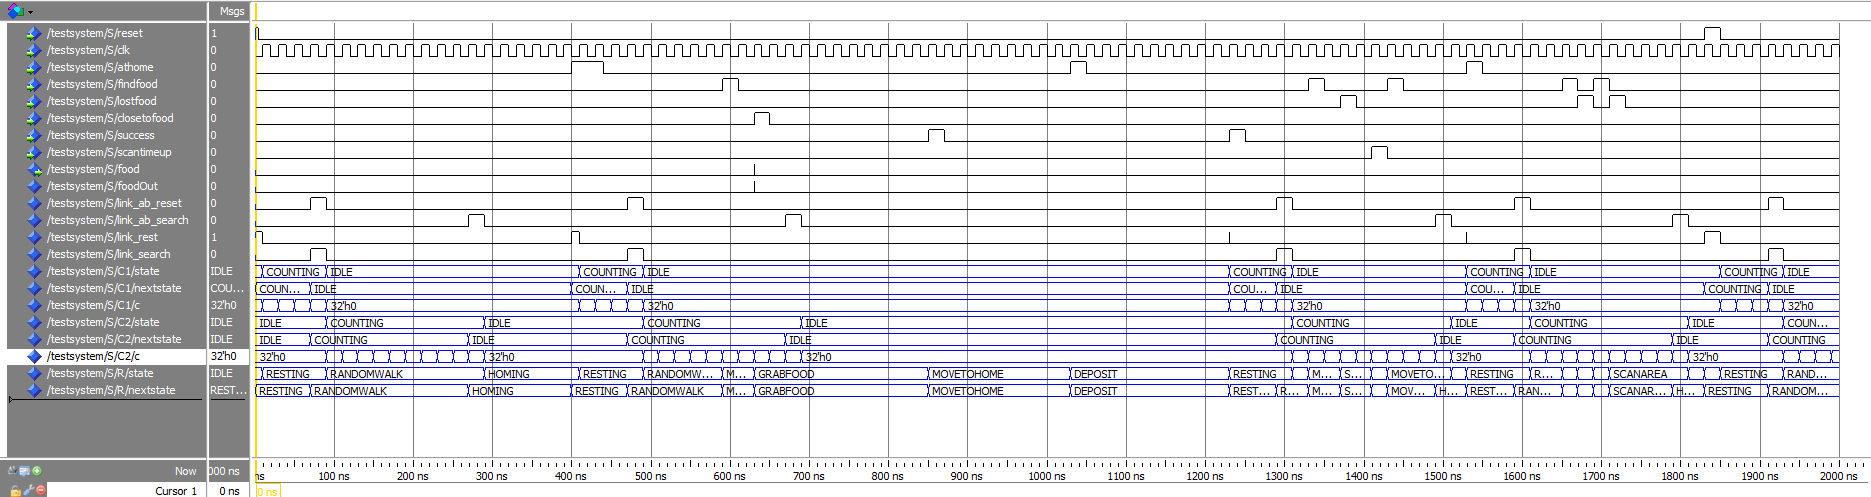
\includegraphics[scale=0.50, angle=-90]{TestSystem.PNG}
\caption{Simulation du Système}
\end{figure}

\begin{figure}[!h]
\advance\leftskip+6cm
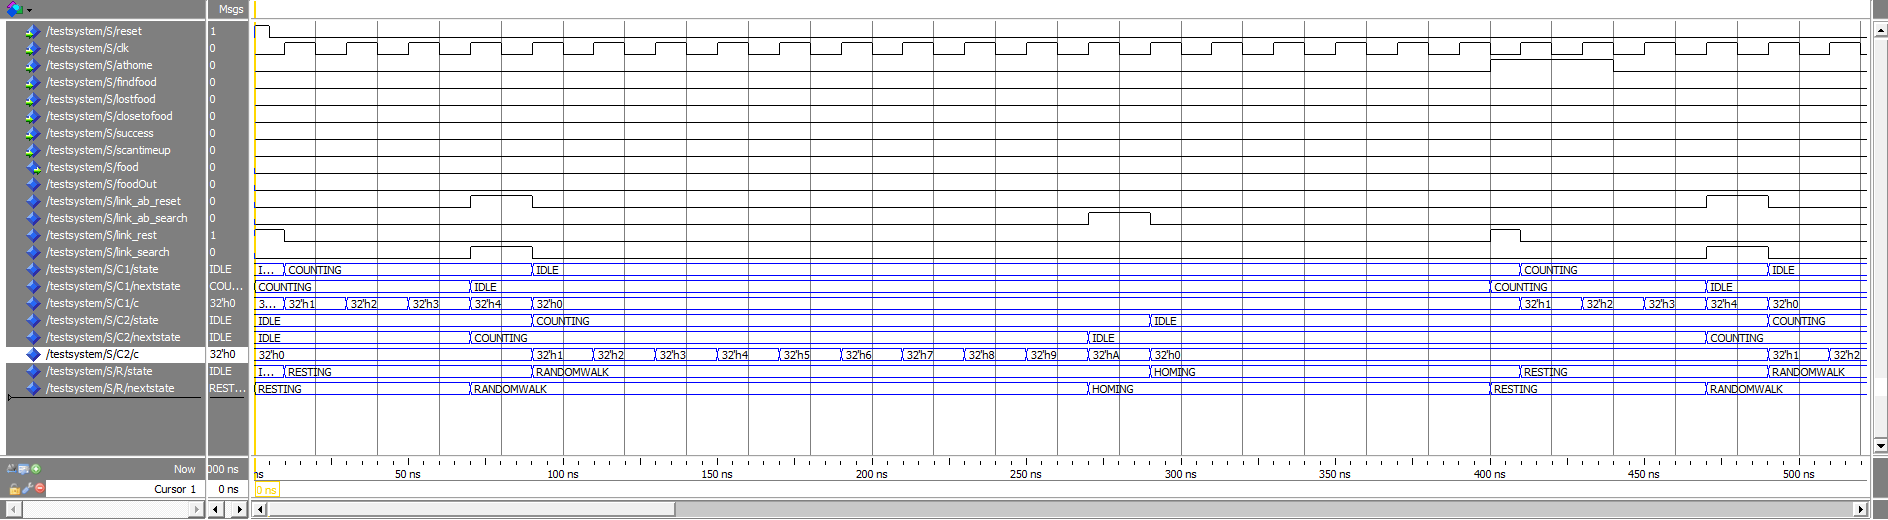
\includegraphics[scale=0.50, angle=-90]{System_detail_part1.PNG}
\caption{Simulation du robot : 0 ns à 500 ns}
\end{figure}

\begin{figure}[!h]
\advance\leftskip+6cm
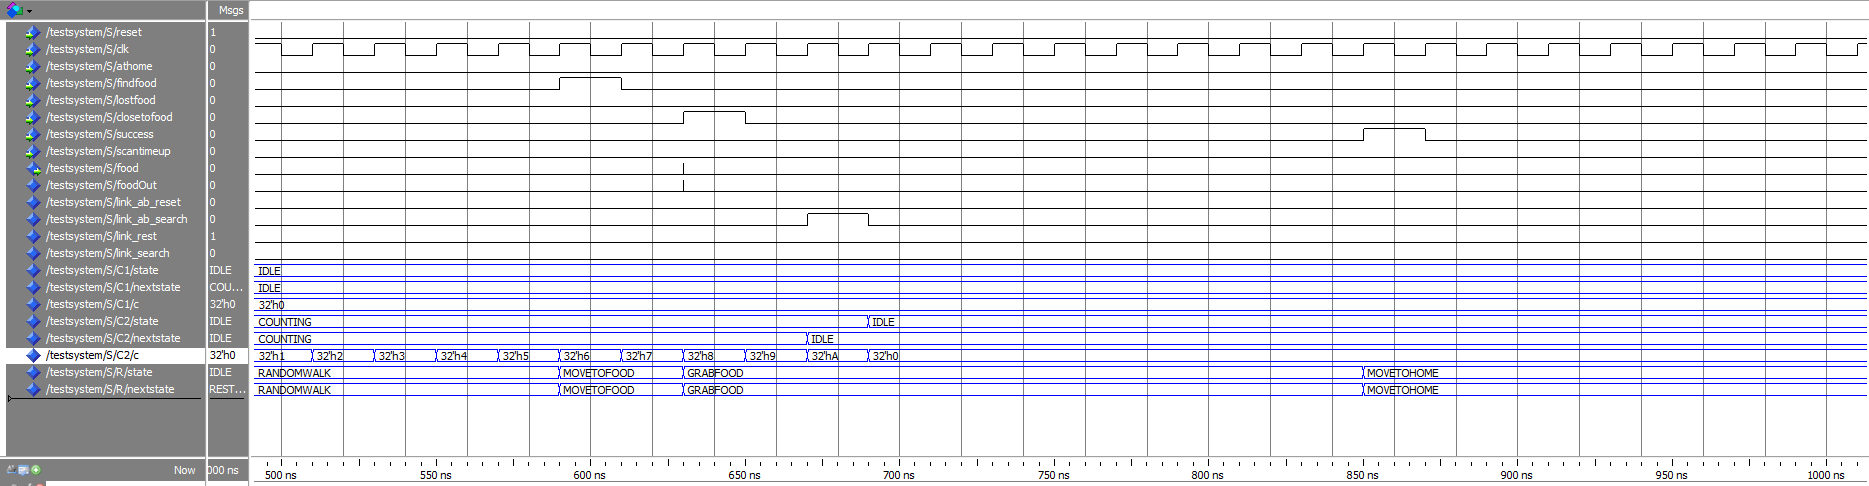
\includegraphics[scale=0.50, angle=-90]{System_detail_part2.PNG}
\caption{Simulation du robot : 500 ns à 1000 ns}
\end{figure}

\begin{figure}[!h]
\advance\leftskip+6cm
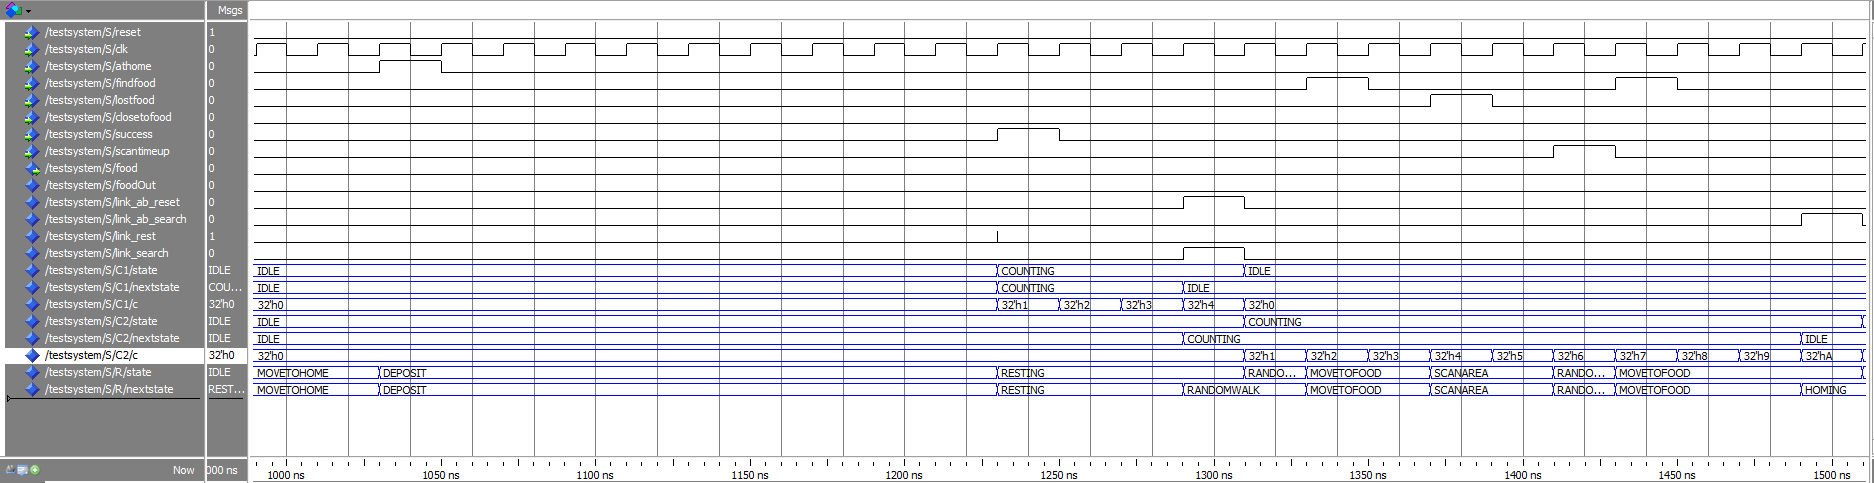
\includegraphics[scale=0.50, angle=-90]{System_detail_part3.PNG}
\caption{Simulation du robot : 1000 ns à 1500 ns}
\end{figure}

\begin{figure}[!h]
\advance\leftskip+6cm
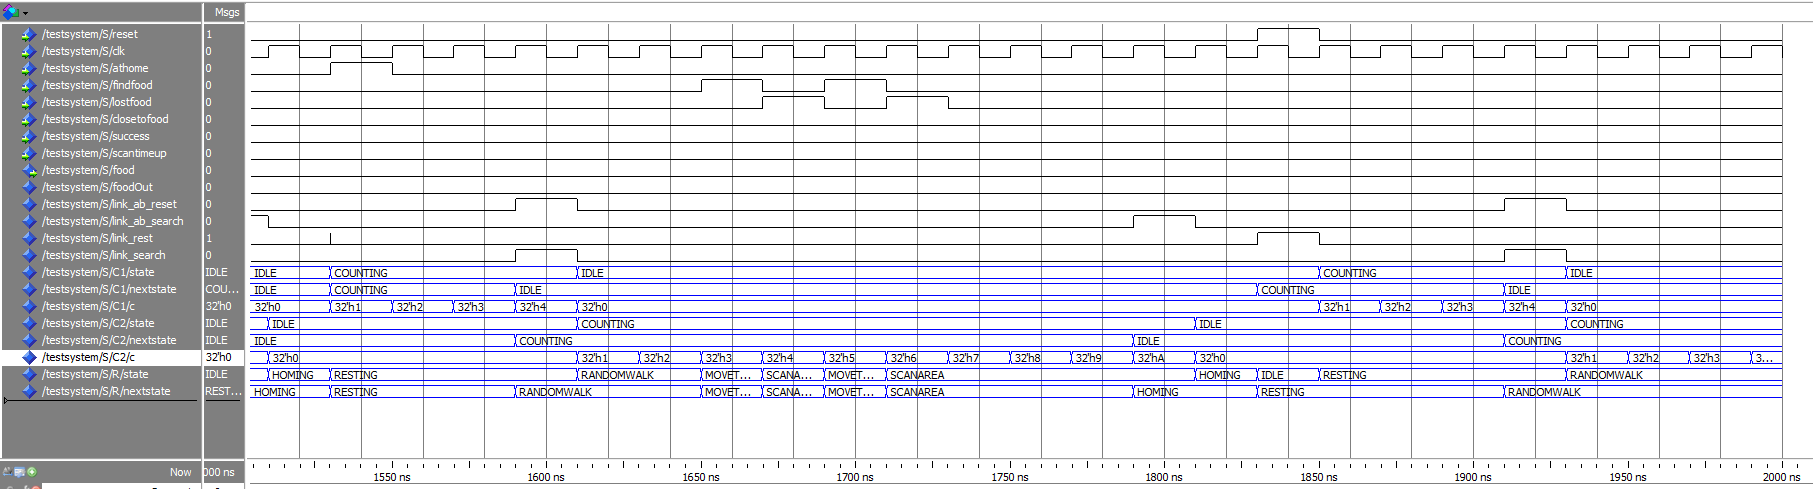
\includegraphics[scale=0.50, angle=-90]{System_detail_part4.PNG}
\caption{Simulation du robot : 1500 ns à 2000 ns}
\end{figure}


\end{document}